
Due to the properties of the Fisher-Rao metric, we can formally decompose the distance
between two functions of $\mathcal{F}$ into the part due to phase and amplitude.

\begin{figure}[Rotation in complex plane]{FIG:ROTATION}{Rotation in complex plane}
	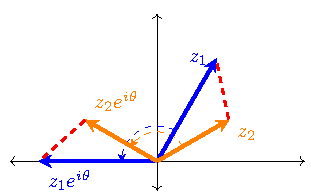
\includegraphics[width=7cm]{rotation}
\end{figure}

Firstly, it is useful to consider and analogy with the rotations on the complex
plane, to understand the role by the phase and the amplitude in the manifold
$\mathcal{F}$.

Let $z_1, z_2$ be two points in $\mathbb{C}$, as it is illustrated in the
Figure \ref{FIG:ROTATION}, when a rotation on the plane is applied the distance
between $z_1$ and $z_2$ remains invariant, i.e., it is an action by isometries, as the
reparameterizations on our manifold.

The variability between two vectors in the plane is completely specified by
the angle between them, which will play the role of the phase in our space, and
the difference of their modules, which will be equivalent to the distance
between the vector once aligned.

\begin{figure}[Phase and amplitude in the complex plane]{FIG:COMPLEX}{Phase and amplitude in the complex plane}

\subfigure[SBFIG:COMPLEX2]{Angle between vectors}{

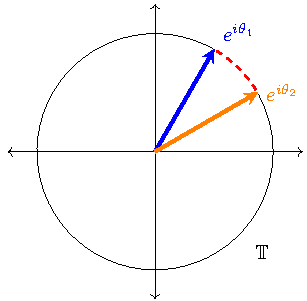
\includegraphics[height=5.5cm]{angle}
} \qquad
\subfigure[SBFIG:COMPLEX2]{Distance in $\mathbb{C}/\mathbb{T}$}{
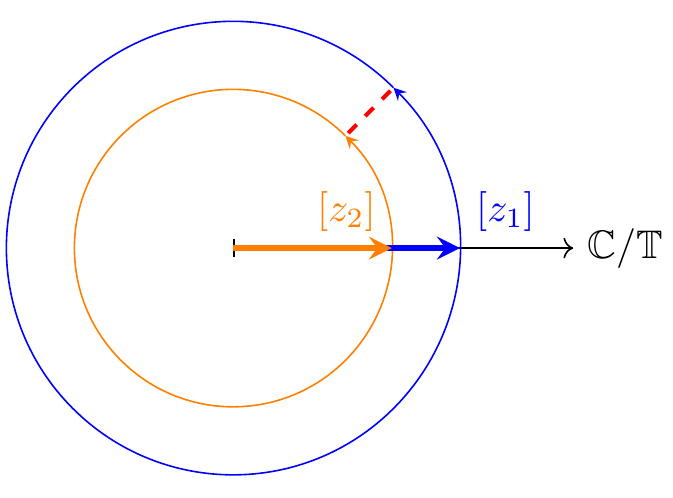
\includegraphics[height=5.5cm]{module}
}

\end{figure}


This distance of the vectors aligned may be understood as a distance in the
quotient space $\mathbb{C} / \mathbb{T}$, where $\mathbb{T}$ is the unit circle,
which it is isomorph to the group of rotations in the plane $SO(2)$. In this
quotient space we will define the equivalence classes
$[z] = \{z e^{i \theta} : \theta \in [0, 2\pi]\}$.

In the case of our manifold, let $q \in \mathbb{L}^2$ be a  \acs{SRSF}. We will define
its orbit under $\Gamma$ as \\$[q] = \{(q, \gamma) : \gamma \in \Gamma \}$, in
other words, it is the set of reparameterizations associated to q. In the
Figure \ref{SBFIG:ORBIT1} it is shown some reparameterizations associated  to a function
of $\mathscr{F}$ and their corresponding SRSF's in \ref{SBFIG:ORBIT2}.


\begin{figure}[Functions in the same orbit]{FIG:ORBIT}{Functions in the same orbit}
  \subfigure[SBFIG:ORBIT1]{$f \circ \gamma_i$}{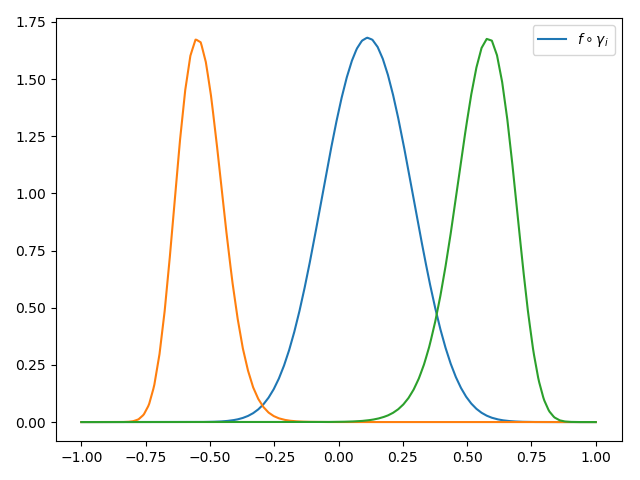
\includegraphics[width=7cm]{orbit-f}} \quad
  \subfigure[SBFIG:ORBIT2]{$(q,\gamma_i)$}{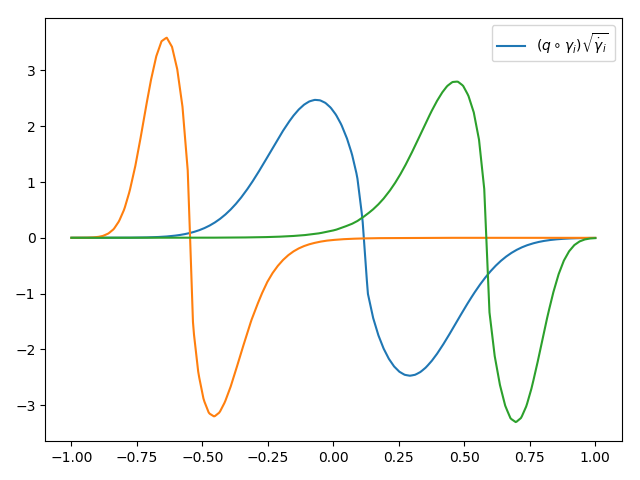
\includegraphics[width=7cm]{orbit-q}}
\end{figure}

We will denote amplitude space $\mathscr{A}= \mathbb{L}^{2} / \Gamma$  to the
set of these orbit. In this space the phase variation is incorporated within
equivalence classes, while the amplitude variation appears across equivalence
classes, as in the analogy with the complex plane. We will endow the space with
the elastic metric, defined as

\begin{equation}[EQ:ELASTIC]{Elastic distance}
d_{a}\left(\left[q_{1}\right],\left[q_{2}\right]\right)=\inf _{
\gamma_{1}, \gamma_{2} \in {\Gamma}}\left(\left\|\left(q_{1},
 \gamma_{1}\right)-\left(q_{2}, \gamma_{2}\right)\right\|\right),
\end{equation}

To quantify the other source of variability, we will define the phase space,
which will denoted as
$\Gamma = \{\gamma :[0,1] \rightarrow[0,1]  : \gamma \text{ is a boundary-preserving diffeomorphism}\}$,
for which the natural distance will be given by the Fisher-Rao metric.

Let $\gamma \in \Gamma$ be a warping function. Under the Fisher-Rao metric,
the norm of such $\gamma$ is 1, thus

\begin{equation}[]{Norm of warping}
\| \gamma \|_\Gamma^2 = \| SRSF(\gamma)\|_{\mathbb{L}^2}^2 =  \| \dot \gamma\|_{\mathbb{L}^2}^2 =
\int_0^1 \sqrt{\dot \gamma (t)} \sqrt{\dot \gamma (t)}dt =
\int_0^1 \dot \gamma(t)dt = \gamma(1) - \gamma(0) = 1.
\end{equation}

The  \acs{SRSF} transform is an isometry between $\Gamma$ and the unit sphere in
$\mathbb{L}^2$, also known as Hilbert Sphere
$\mathbb{S}_\infty = \{ \psi \in \mathbb{L}^2 : \|\psi\|_{\mathbb{L}^2}=1\}$.
To calculate distances in $\Gamma$ we will apply this transformation which will
allow us to take advantage of the structure of $\mathbb{S}_\infty$.

Let $\gamma_1, \gamma_2$ be in $\Gamma$ and $\psi_1=\sqrt{\dot \gamma_1},
\psi_2=\sqrt{\dot \gamma_1}$ be their  \acs{SRSF}, their distance in $\Gamma$ will be
given by

\begin{equation}[]{Phase distance}
d_{phase}(\gamma_1, \gamma_2) = d_{\psi}(\psi_1, \psi_2) =
\cos^{-1}\left (\int_0^1 \psi_1(t) \psi_2(t) dt\right ).
\end{equation}

This result is analogous to the rotations in the plane, where the cosine of
the angle between two unit vectors will be given by the inner product.
If we apply a rotation to two vectors, their angle remains invariant, in our
case the phase distance will be invariant to common reparameterizations due to
the properties of the Fisher-Rao metric.

Let $f_1, f_2$ be functions in $\mathcal{F}$, their relative phase is defined as

\begin{equation}[EQ:RELATIVEPHASE]{Relative phase}
\left(\gamma_{1}^{*}, \gamma_{2}^{*}\right)=\underset{\gamma_{1}, \gamma_{2} \in \Gamma}{\operatorname{argmin}}\left\|\left(q_{1}, \gamma_{1}\right)-\left(q_{2}, \gamma_{2}\right)\right\| \in \Gamma \times \Gamma.
\end{equation}

Thus allow us to calculate the phase variability between them,
as a generalization of the notion of an angle. The phase distance between these
functions is the distance of their relative phase
$d_{phase} (\gamma_{1}^{*}, \gamma_{2}^{*})$. Alternatively, the properties of
the metric can be used to define the relative phase depending on a single warping,
$
\gamma_{12}^{*}=\underset{\gamma \in \Gamma}{\operatorname{argmin}}\left\|\left(q_{1}, \gamma \right)- q_{2}\right\|,
$
which is quivalent to set $\gamma_2^*$ to the identity in \ref{EQ:RELATIVEPHASE}.
